\documentclass{article}
\usepackage[utf8]{inputenc}

%\usepackage[md]{titlesec}
\usepackage{graphicx}

\usepackage[export]{adjustbox}

\usepackage{subcaption}

\setcounter{tocdepth}{1}

\renewcommand{\thesubsection}{\alph{subsection}}
%\renewcommand{\thesubsubsection}{\arabic{\subsubsection}}



\date{October 21, 2016}


\title{\textbf{Assignment 8}\\Configuring Virtual Trunking Protocol & Troubleshooting}
\author{s316620}


\begin{document}

\maketitle
\newpage

\section{Basic VLAN} 
Implementing the VLAN topology show in Figure \ref{fig:topassign}, and configuring it to the specifications outlined in Table \ref{tab:topology1-config}. 
\begin{table}[h]
    \centering
    \begin{tabular}{|c|c|c|c|}
    \hline
    Device & VLAN & VLAN name & IP address \\
    \hline
    SW-1& & & None \\
         SW-2& & & None \\
         H1 & 10 & Student & 192.168.10.1/24\\
         H2 & 10 & Student & 192.168.10.2/24\\
         H3 & 20 & Staff & 192.168.20.3/24\\
         H4 & 10 & Student & 192.168.10.4/24\\
         H5 & 20 & Staff & 192.168.20.5/24 \\
         H6 & 30 & Admin & 192.168.30.6/24 \\
         H7 & 30 & Admin & 192.168.30.7/24 \\
         \hline
    \end{tabular}
    \caption{Set-up configurations for topology 1 (from Assignment 8). }
    \label{tab:topology1-config}
\end{table}

In PacketTracer we use generic hosts for the hosts and a generic switch for the switches. The connection between the hosts and the switches were done using copper straight cables and the connection between the switches was done using the crossover cable. In the Switches we add the VLAN's as seen in Figure \ref{fig:1vlanconf}. 
We configure the IP addresses for each of the hosts.
\begin{figure}[h]
    \centering
    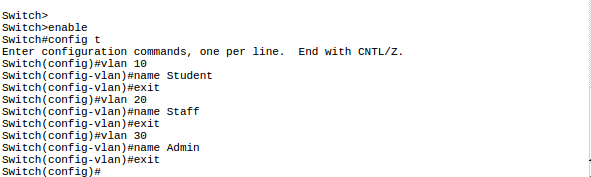
\includegraphics[scale=0.6]{1vlanconf}
    \caption{Adding the VLANs in the switches.}
    \label{fig:1vlanconf}
\end{figure}

We configure the interfaces for the switches, the switch's port connected to the hosts have \textit{switchport mode access} and the ports connecting the switches to each other have \textit{switchport mode trunk}. The port is configured to be \textit{trunk} as shown in Figure \ref{fig:1trunkconf} and then we configure the \textit{access} ports with vlan as shown in Figure \ref{fig:1accessconf}.

\begin{figure}[h]
    \centering
    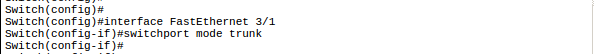
\includegraphics[width=\textwidth]{1trunkconf}
    \caption{Configuring \textit{trunk} port.}
    \label{fig:1trunkconf}
\end{figure}

\begin{figure}[h]
    \centering
    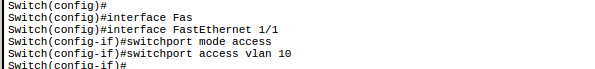
\includegraphics[width=\textwidth]{1accessconf}
    \caption{Configuring \textit{access} port with VLAN.}
    \label{fig:1accessconf}
\end{figure}

We see that there is connection only between hosts in the same VLAN and the hosts in different VLAN have no connectivity, we \textit{ping} from H1 (192.168.10.1) to H4 (192.168.10.4) which has connectivity as it is in the same VLAN and from H1 (192.168.10.1) to H3 (192.168.20.3) which does not have connectivity as it is in different VLANs, as seen in Figure \ref{fig:1ping}. 

\begin{figure}[h]
    \centering
    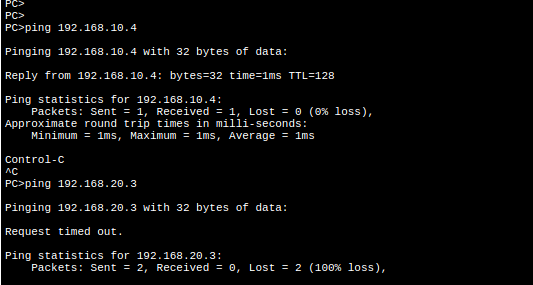
\includegraphics[scale=0.4,width=0.8\textwidth]{1ping}
    \caption{Checking connectivity between hosts from H1 to H4 (same VLAN) and H1 to H3 (different VLAN).}
    \label{fig:1ping}
\end{figure}

This configurations implemented in Packet Tracer can be seen in Figure \ref{fig:1pt}

\begin{figure}[h]
    \centering
    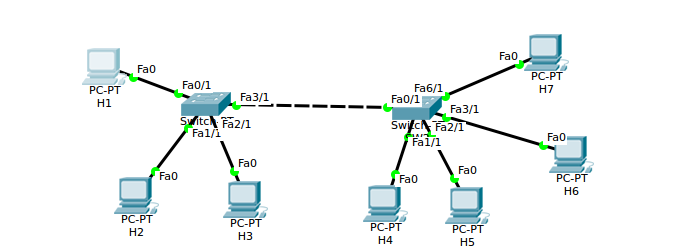
\includegraphics[scale=0.4,width=\textwidth]{1pt}
    \caption{Topology in PacketTracer}
    \label{fig:1pt}
\end{figure}

\section{ More VLANs in Packet Tracer}

\begin{table}[h]
    \centering
    \begin{tabular}{|c|c|c|}
    \hline\\
    Device & VLAN & IP address \\
         Switch-A& - & None \\
         Switch-B& -& None \\
           Switch-C& - & None \\
         PC-10 & VLAN 10 & 10.0.0.1/24\\
         PC-20 & VLAN 20 & 10.0.0.2/24\\
         PC-11 & VLAN 10 & 10.0.0.3/24\\
         PC-21 & VLAN 20 & 10.0.0.4/24\\
         \hline
    \end{tabular}
    \caption{Set-up configurations for topology 2 (from Assignment 8). }
    \label{tab:topology2-config}
\end{table}

\subsection{Setting up the topology in PacketTracer}

Setting up  the topology as seen in Figure \ref{fig:topology2-config} in PacketTracer with the configurations seen in Table \ref{tab:topology2-config}. We add VLAN name 'Administration' with VLAN tag number '10' and VLAN with name 'Students' and tag number '20' in all the switches. We can see this is configured using the \textbf{show vlan} command as seen in Figure \ref{fig:2showvlan}. 

\begin{figure}[h]
    \centering
    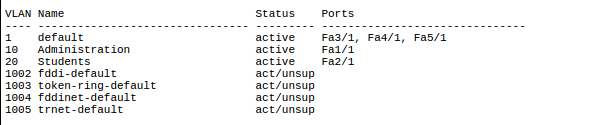
\includegraphics[scale=0.5]{2showvlan}
    \caption{The \textbf{show vlan} command in the switch.}
    \label{fig:2showvlan}
\end{figure}

\begin{figure}
    \centering
    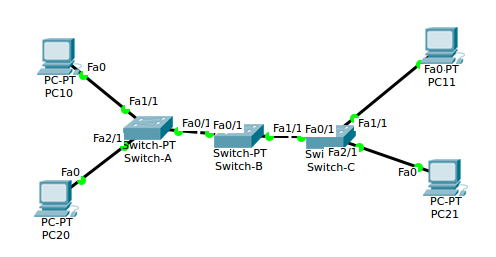
\includegraphics[scale=0.3,width=0.8\textwidth]{topology2-config}
    \caption{Topology 2 in PacketTracer from Assignment 8}
    \label{fig:topology2-config}
\end{figure}

\subsection{Connectivity between hosts}

Checking the connectivity between hosts with the \textbf{ping} command, we ping from PC-10 to all other hosts and from PC-20 to all other host. Before configuring the VLAN in the switch ports we can connect from each hosts to all other. But after configuring the VLAN we only have connection between the hosts in the same VLAN as seen in Figure \ref{fig:2ping}.

\begin{figure}[h]
    \centering
    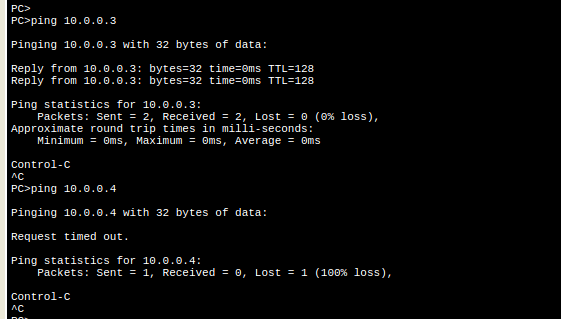
\includegraphics[scale=0.5]{2ping}
    \caption{Checking connectivity between hosts}
    \label{fig:2ping}
\end{figure}

\subsection{Temporarily suspend access to PC-11}

To temporarily restrict access to the VLAN we can use the command :\\ \textbf{switchport trunk allowed vlan except \textless\textit{VLAN ID}\textgreater} to restrict access to VLAN. This command is run in the \textit{trunk} port of the switch the host is connected to.

\section{Virtual Trunking Protocol (VTP)}

Imagine that you have to configure 100 switches with
10 different VLANs. Definitely , it will take way too much time
to configure these switches and it will be impossible for 
making multiple changes for all of them at once. This is why the use of VTP is convenient 
in big environments. VTP is a protocol used for distributing VLANs configured on 
switches through trunk links. It can operate in 3 modes, namely :
\begin{enumerate}
    \item  Server             
    \item Client
    \item Transparent
\end{enumerate}

The switch configured in the server mode is where the VLANs are configured and the information gets distributed from the Server switch (\textit{usually in the core}) to the switches working in client mode (\textit{usually the access switches}). There can be multiple switches in the server mode all having the same VLAN configuration and they will be interchanging VLAN data. In order to keep the VLAN database consistent, there is a parameter called \textit{Configuration Revision} and each time you make a VTP configuration change this parameter will get incremented. All switches will aplly the configuration with the currently highest \textit{Configuraton Revision} number. The third mode name \textit{transparent} for which the switches can be configured is used to forward VLAN data, but without applying the VLAN changes on the local switch. VTP can be configured to work in different domains, but for the purpose of this assignment we will stick to using a single VTP domain. In order for the switches to exchange VLAN data, the switches need to have the same VTP domain and VTP password configured.

\subsection{Setting up Topology 3 in Packet Tracer}

I set up topology 3 as seen in Figure \ref{fig:3top}. Then I configure all the ports between the switches to run in trunking mode using the \textbf{switchport mode trunk}
command. 
\begin{figure}[h]
    \centering
    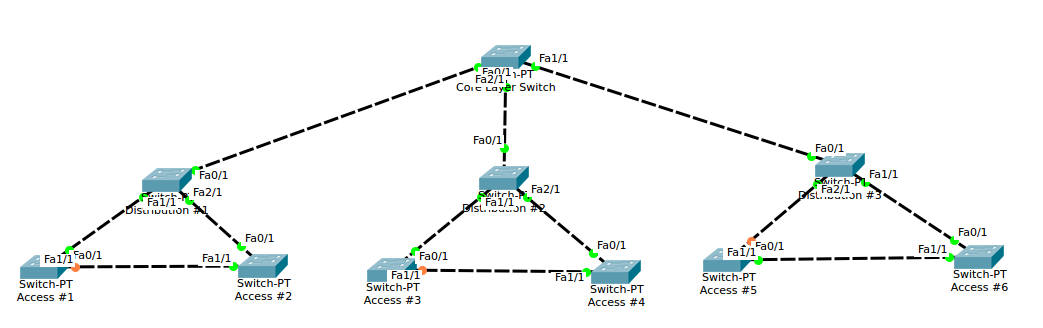
\includegraphics[scale=0.4,width=\textwidth]{3top}
    \caption{Topology 3 in Packet Tracer}
    \label{fig:3top}
\end{figure}

\subsection{Configuring VTP}

As default all the switches are running in server mode. Now the distribution switches will run in the \textit{transparent mode}, this is done as seen in Figure \ref{fig:vtptransparent}. The access switches are running in the \textit{client mode} this can be seen in Figure \ref{fig:vtpclient}. 

\begin{figure}[h]
\centering
    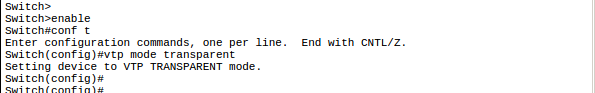
\includegraphics[width=\textwidth]{vtptransparent}
    \caption{Configuring the switch to \textit{transparent mode}.}
    \label{fig:vtptransparent}
\end{figure}
    
\begin{figure}[h]
\centering
    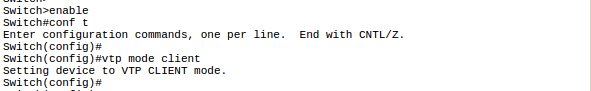
\includegraphics[width=\textwidth]{vtpclient}
    \caption{Configuring the switch to \textit{client mode}.}
    \label{fig:vtpclient}    
\end{figure}


\subsection{Configuring the VTP domain}

We configure the VTP domain on all the hosts with the \textbf{vtp domain \textless \textit{domain name}\textgreater}, in the \textit{configure mode}, where the \textit{domain name} used is my student ID. 

\subsection{Setting up security}
To configure the password we use the command \textbf{vtp password 123}, this is done on all the switches. 

\subsection{Creating VLANs}

Now the VLAN will be created locally only at the \textit{core switch}, using the same procedure as seen in previous tasks. We use the following VLAN tags : 
\begin{enumerate}
    \item \textit{Administration} - VLAN 10 
    \item \textit{Students} - VLAN 20
    \item \textit{IT} - VLAN 30
\end{enumerate}

\subsection{Observations}

\begin{enumerate}
    \item \textit{Which VLANs do you observe in the ouput in the core switch?}\\
    In the core switch we can see the \textit{Administration}, \textit{Students} and \textit{IT} VLAN. It is running the the \textit{core} VTP mode.
    
    \item \textit{Which VLANs do you observe in the ouput in the distribution switch?}\\
        In the distribution switches we cannot see the VLANs that we added. It is in the \textit{transparent} mode. 
        
    \item \textit{Which VLANs do you observe in the ouput in the access switch?}\\
        In the access switches we can  see the VLANs that we added. It is in the \textit{client} mode. 
\end{enumerate}   

\subsection{Adding hosts}

Then we add hosts to the topology and configure the access ports on the access layer switches according to the table in Figure \ref{fig:tabletop}

\begin{figure}[!h]
    \centering
    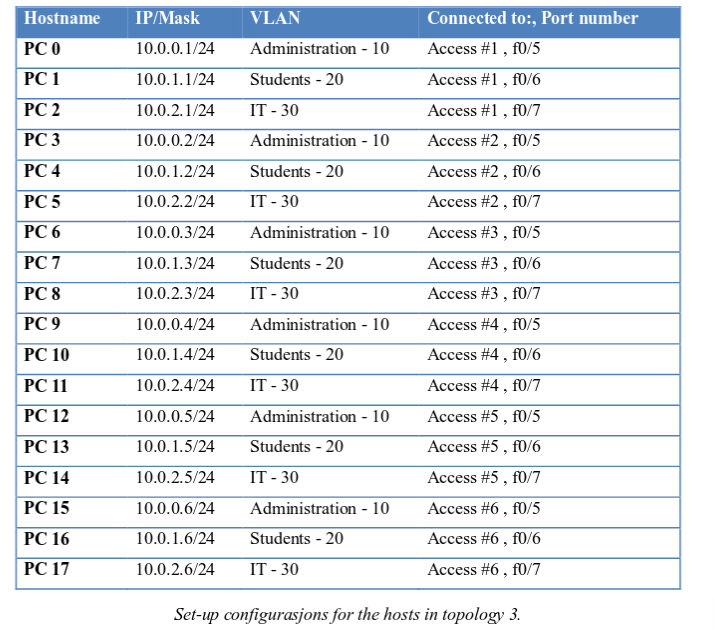
\includegraphics[scale=0.6,width=0.8\textwidth]{3tabletop}
    \caption{}
    \label{fig:tabletop}
\end{figure}

\subsection{Redundancy}

Now we can observe that there is connectivity only between the hosts in the same VLAN. If we ping from PC0(10.0.0.1) to PC3(10.0.0.2) we have connectivity , but if ping from PC3(10.0.0.2) to PC6(10.0.0.3) we do not have connectivity, as there are no local VLANs created on the distribution layer switches. We have to connect switch Access\#2 to Access\#3 and Access\#4 to Access\#5, and set those links into trunking mode. Save the configurations persistently with the \textbf{write} command or \textbf{copy running-config startup-config} command,  and then save the packet tracer file.


\section{More Virtual Trunking Protocol(VTP) and VLAN.}

In this task, I configure a VLAN according the specification in Table \ref{tab:topospecs} and configure the VTP on the middle switch (SW-3). Our topology can be seen in Figure \ref{fig:acttopo}. The connection between the hosts and the switches is done by using the \textit{straight} cable and the connection between the switches is done using the \textit{crossover} cable. 

\begin{figure}[!h]
    \centering
    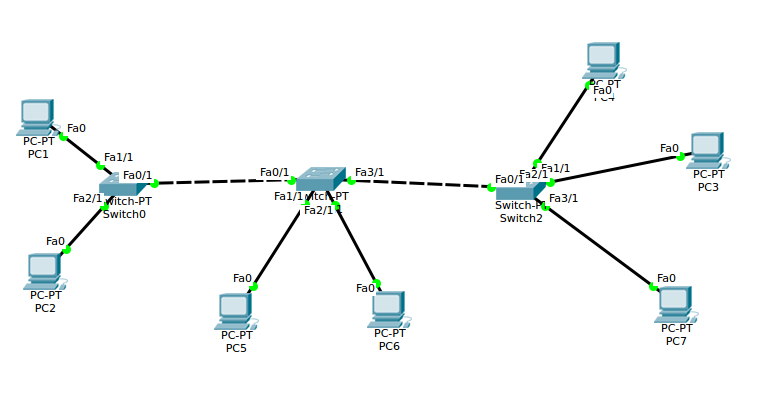
\includegraphics[scale=0.6,width=\textwidth]{acttopo}
    \caption{Topology in PacketTracer}
    \label{fig:acttopo}
\end{figure}

The topology is seen in PacketTracer. The connection port between the switches is in \textit{trunk} mode and the switch ports connected to the hosts have access. VTP was set up as seen in the previous tasks. The VTP domain and password used are s316620 and 123 respectively.  The center switch is in the Server mode ,and the other two switches are in the Client mode. 


\begin{table}[h]
    \centering
    \begin{tabular}{c|c|c}
    \hline
         Device &  VLAN & IP address\\
        \hline
         PC-1 & 10 & 192.168.1.2 \\
         PC-2 & 40 & 192.168.4.2 \\
         PC-3 & 20 & 192.168.2.2 \\
         PC-4 & 20 & 192.168.2.3 \\
         PC-5 & 40 & 192.168.4.3 \\
         PC-6 & 30 & 192.168.3.2\\
         PC-7 & 10 & 192.168.1.3 \\
         \hline
    \end{tabular}
    \caption{Figure \ref{fig:acttopo} topology specifications.}
    \label{tab:topospecs}
\end{table}


\section{Router-on-stick}

As it is not possible for different VLANs with different masks to communicate. We configure a router-on-stick that will enable all of the VLANs to communicate freely, we set up InterVLAN connectivity.  As seen in Figure \ref{fig:routerconf} we add sub-interfaces to interface connected to the switch at the Router. Then connect the switch and router using the straight cable, and set the port at Switch which is connected to the Router to \textit{trunk} mode.  


\begin{figure}[h]
    \centering
    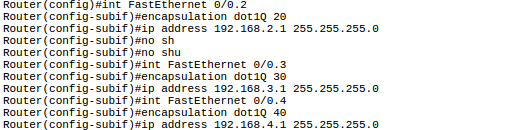
\includegraphics[width=\textwidth]{5routerconf}
    \caption{}
    \label{fig:routerconf}
\end{figure}

After doing this although I could ping from Hosts to the Router and vice versa, I could not ping between hosts on  different VLAN. 

 
 My \textit{running-config} at the center looks as follows:
\begin{verbatim}
Switch#show running-config 
Building configuration...

Current configuration : 657 bytes
!
version 12.1
no service timestamps log datetime msec
no service timestamps debug datetime msec
no service password-encryption
!
hostname Switch
!
spanning-tree mode pvst
!
interface FastEthernet0/1
 switchport mode trunk
!
interface FastEthernet1/1
 switchport access vlan 40
 switchport mode access
!
interface FastEthernet2/1
 switchport access vlan 30
 switchport mode access
!
interface FastEthernet3/1
 switchport mode trunk
!
interface FastEthernet4/1
!
interface FastEthernet5/1
!
interface FastEthernet6/1
 switchport mode trunk
!
interface Vlan1
 no ip address
 shutdown
!
line con 0
!
line vty 0 4
 login
line vty 5 15
 login
!
end
\end{verbatim}


And my \textit{running-config} at the router looks like : 

\begin{verbatim}
Router#show running-config 
Building configuration...

Current configuration : 1053 bytes
!
version 12.2
no service timestamps log datetime msec
no service timestamps debug datetime msec
no service password-encryption
!
hostname Router
!
ip cef
no ipv6 cef
!
interface FastEthernet0/0
 no ip address
 duplex auto
 speed auto
!
interface FastEthernet0/0.10
 encapsulation dot1Q 10 native
 ip address 192.168.1.1 255.255.255.0
!
interface FastEthernet0/0.20
 encapsulation dot1Q 20
 ip address 192.168.2.1 255.255.255.0
!
interface FastEthernet0/0.30
 encapsulation dot1Q 30
 ip address 192.168.3.1 255.255.255.0
!
interface FastEthernet0/0.40
 encapsulation dot1Q 40
 ip address 192.168.4.1 255.255.255.0
!
interface FastEthernet1/0
 no ip address
 duplex auto
 speed auto
 shutdown
!
interface Serial2/0
 no ip address
 shutdown
!
interface Serial3/0
 no ip address
 shutdown
!
interface FastEthernet4/0
 no ip address
 shutdown
!
interface FastEthernet5/0
 no ip address
 shutdown
!
ip classless
!
ip flow-export version 9
!
line con 0
!
line aux 0
!
line vty 0 4
 login
!
end
\end{verbatim}

\end{document}

